%!TEX root = ../BoYu-Dissertation.tex
\graphicspath{{Figures/}}

\chapter{Introduction} 
\label{chapter1:introduction}

\section{Problem Scope}
Support for awareness is one of the most active research areas in computer supported cooperative work (CSCW) \cite{dourish1992awareness,schmidt2002a,rittenbruch2009a}. At its essence, awareness refers to the ability of collaborators to understand each others' activities and relate them to a joint context \cite{rittenbruch2009a}. This context is essential for collaboration as it is used to ensure that individual contributions are relevant to the group’s activity as a whole, and allow groups to coordinate the process of collaborative working \cite{dourish1992awareness}.  

One general design concern for awareness systems is that awareness must be achieved with minimal attention and effort from the participants of teamwork \cite{markopoulos2009design}. Awareness falls into the category of `the articulation work' that is required for coordination but not the primary goals for collaboration  \cite{schmidt1992taking}. Taking extra time and effort to achieve awareness can interrupt the current line of action, and therefore damage team performance \cite{fussell1998coordination}. As a result, a large number of awareness mechanisms and tools have been proposed in the literature, aiming at promoting awareness in a relatively effortless way \cite{rittenbruch2009a}.

Although much progress has been made in designing awareness mechanisms to support team activity at relatively small and medium scales \cite{antunes2010a}, it becomes a much more difficult task to promote awareness in complex and highly distributed activities \cite{cabitza2009promoting}. The geo-collaborative activities of interest in this study are a subset of these complex collaborative setting, where awareness is unlikely to be achieved effortlessly, and hence it becomes even more important to design computational artifacts that actively promote awareness. In the rest of this section, we first describe the characteristics of collaborative settings that we consider as geo-collaboration in this study, and then present the challenges for supporting awareness in geo-collaboration that motivates our work.

\subsection{Geo-Collaboration} % (fold)
\label{sub:geo_collaboration}
\fxerror{How we define complexity: 1. distributed in geography, 2. number of activities and dependencies, 3. task-specific asymmetries among actors, 4. level of contingency}

The geo-collaborative activities we consider in this paper are a subset of complex collaborative setting, with the following characteristics: 

\begin{enumerate}
\item Multiple team members are geographically distributed.

\item They are engaged in tightly interdependent activities that require effective coordination.

\item They work in dynamic setting that entails rapid and frequent changes in environment and activities. 

\end{enumerate}

Examples of geo-collaboration within these boundaries abound in practical applications such as crisis management, resource management, military exercises, and science explorations. For the ease of illustrating the work we present in this study, we will frequently refer to the following scenario in emergency response.

\begin{scenario}
\textbf{An Emergency Response Scenario.} A chemical factory near an urban area was exploded and caused a major pollution. To respond to this critical incident, task force is formed that includes search and rescue teams, decontamination teams, medical treatment teams, and transportation teams. Teams are dispatched and configured geographically to cover the impacted area. Each team cover a functional area of the overall mission.  Search and rescue teams patrol the incident area to search for victims and report their locations and status. Discovered victims are first decontaminated (by one of the Decontamination teams) before they can be moved to other facilities.  If a victim is wounded, he or she will be scheduled and transported to a medical station for treatment. All transportation needs for moving victims to treatment stations and shelters are handled by the transportation team. Although teams are working autonomously on their local tasks, they must coordinate their capacity, schedule, and priority to deal with emerging and unexpected situations in order to save and protect all the victims in an efficient fashion.
\end{scenario}

Such an emergency situation usually involves multiple individuals and organizations that are distributed in different geographic locations. Figure \ref{fig:scenario_overview} shows a hypothetical distribution of tasks and teams in relation to the disaster area. Because of the distribution, workers structure their tasks so that they can work relatively autonomously within their local environment and responsibilities. In the same time, due to interdependencies among sub-activities \cite{shen2004managing}, they find themselves working on a multitude of different activities, interleaving them in ways that seem best suited for getting their work accomplished given the practical pressures. Furthermore, exceptions to the planned responses are a common and critical factor in these activities \cite{Turoff2004}. What specific information is of concern and interest to a given individual is changing rapidly.

\begin{figure}[htbp] %  figure placement: here, top, bottom, or page
   \centering
   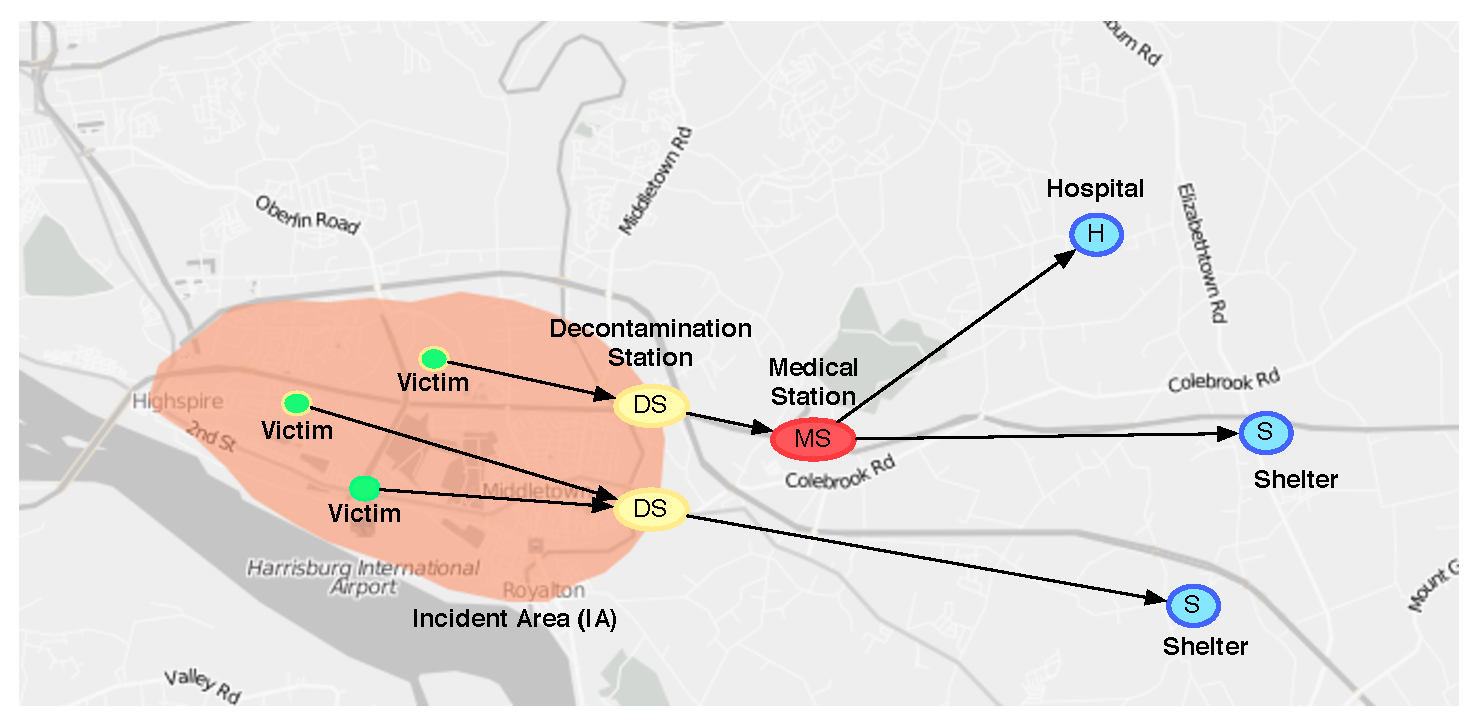
\includegraphics[width=5.8in]{scenario.pdf} 
   \caption{An emergency scenario}
   \label{fig:scenario_overview}
\end{figure}

% subsection geo_collaboration (end)




\subsection{Challenges in coordinating geo-collaboration} % (fold)
\label{sub:challenges_in_coordination}
This scenario clearly demonstrates two major challenges to support awareness in complex geo-collaborative activities: the high level complexity and contingency of collaborative activities.

\fxwarning{This section needs to be updated to more focus on the awareness support.}

\subsubsection{High level of complexity} % (fold)
\label{ssub:high_level_of_complexity}
With low degrees of complexity, the coordination of cooperative work can be achieved by means of mutual awareness and alignment \cite{schmidt2002a}. As demonstrated by the body of rich empirical studies of cooperative work within CSCW \cite{heath2002a}, actors tacitly monitor each other; they perform their activities in ways that support coworkers' awareness and understanding of their work; they take each others' past, present and prospective activities into account in planning and conducting their own work; they gesture, talk, write to each other, and so on, and they mesh these interactional modalities dynamically and seamlessly . This appears effortless, because, to a competent member in the flux of doing the work and thus attuned to the changing state of the field of work — what the colleagues next to him are doing is immediately meaningful; it does not require interpretation, reflection, contemplation to know why they are doing what they are doing or why they are not doing something else \cite{schmidt2002a}.

However, in the complex work settings that characterize modern industrial, service, and administrative organizations where hundreds or thousands of actors engaged in myriads of complexly interdependent activities, the task of coordinating the interdependent and yet distributed activities is of an order of complexity where the mutual awareness mechanisms are far from sufficient. Carstensen’s study of a software development project \cite{carstensen1994we} clearly illustrates the problem of scaling with complexity. In previous projects the systems they had been constructing had been small and the programming work had been done by a couple of programmers. In these projects they had been able to manage their interdependencies practically effortlessly. They had been working next to each other and had practically unconstrained access to consulting each other and to monitoring each other’s work. At the time of the study, however, a new project had been undertaken in which the engineers were building a significantly larger system comprising many hundred thousands lines of code. Their traditional coordinative practices were now quite inadequate. The interdependencies of their cooperative effort now transcended the local practices, and they were faced with situations that the effects of their local activities to other regions of the cooperative effort are not immediately and straightforwardly evident. To deal with the ensuing crisis, the ensemble had to develop a set of formal coordinative artifacts, such as the bug report forms, to regulate local practices.

One of the major challenges demonstrated in the scenario is characterized by the degree of \emph{complexity} of dependencies that can exist in coordination work. With low degrees of complexity (e.g. when the number of dependencies that need to manage is limited, or their effect is only within the scope of local practices), the coordination of collaborative work can be achieved by means of human communicative and cognitive skills \cite{schmidt1996a}. However, in the complex work settings as described in the scenario, multiple dependencies can co-exist at the same time, and they together form a web of dependencies where state changes of one of them can cause chain effects on others. Faced with a high degree of complexity of coordination work, collaborative actors often use a category of symbolic artifacts which, in the context of a set of procedures and conventions, stipulate and mediate coordination work and thereby are instrumental in reducing its complexity and in alleviating human effort \cite{simone1995notation}. These artifacts, together with the concomitant procedures and conventions are called `coordination mechanisms' \cite{schmidt1996a}. The first goal of this study aims at building an integrated coordination mechanism that would keep track of the state of work and to manage relations and dependencies among actors, tasks, and resources in order to reduce the complexity of coordination work in geo-collaborative activities.
% subsubsection high_level_of_complexity (end)

\subsubsection{High level of contingency} % (fold)
\label{ssub:high_level_of_contingency}
Developing appropriate coordination mechanisms must be based on a solid understanding of various collaborative dependencies, i.e. the capabilities of coordination mechanisms should match coordination requirements of the task at hand. In relatively static work domains such as process control or manufacturing, the set of work dependencies is largely known in advance and thus it becomes feasible to specify formal coordination mechanisms to manage them, such as routines, pre-planning, or standardization. Increasingly, however, collaborative work is characterized by high levels of interdependence, uncertainty, and time constraints, such as cooperative design \cite{carstensen1994we} or emergency response \cite{shen2004managing}. In these dynamic contexts, interdependence of work is emerging and rapidly shifting over time \cite{espinosa2004explicit}. Due to changes and evolution of collaborative plans, dependencies may emerge, sustain, or disappear as the activity advances. 

The contingency of dependencies can be clearly evidenced in the motivating scenario, where patterns of dependencies among people are in fact quite volatile, either due to the changes of environment in which the work is done (environmental uncertainty), or the changes of the task that the contributors are trying to accomplish (task uncertainty) \cite{kittur2009coordination}. For instance, while the decontamination process at a given decontamination station is under way, a first responder reports that five new victims have been discovered and are on their way to the decontamination station. As a result, a request to deliver an additional operator is initiated in anticipation of exceeding its maximum capacity of victims the station can handle. Suddenly, the decontamination process becomes intertwined with the process of delivering the operator, and the five new victims cannot be decontaminated until the new operator arrives at the station. In this way, such unexpected events cause seemingly un-related tasks to suddenly become interdependent.

As a result, we believe that the contingency in the interdependence of work represents a major feature of complex geo-collaborative work, but existing coordination tools have not taken this into account seriously. When a collaborative activity involves an extended period of work with volatile dependencies, the potential dependencies (i.e. the collective set of all dependencies that could potentially happen during the whole activity) are a quite large number, but the actual dependencies (i.e. those dependencies that are live and need to be coordinated) are rather a relatively small number. Coordination tools could play a more effective role if they target coordination of actual dependencies, rather than potential dependencies. However, identifying the set of actual dependencies at any given moment is difficult due to the fact that such dependencies are unknown a priori and they emerge as a consequence of the evolving activity. It would be highly desirable for collaborative tools to be able to assess the characteristics of the activities, computationally identify actual dependencies, and track their changes over time. 
% subsubsection high_level_of_contingency (end)
% subsection challenges_in_coordination (end)
% section motivation (end)


\section{Research Objectives and Approach} % (fold)
\label{sec:research_objectives}
By setting the scene in the previous section, the overall objective of this dissertation is to addresses the major challenges in coordinating complex, dynamic, and distributed geo-collaborative activities by developing an awareness-based coordination mechanism that can utilize the knowledge of activities and dependencies.

To achieve the research objective, this study follows the design science paradigm in information systems research \cite{Hevner2004}. Knowledge and understanding of the aforementioned coordination problems in geo-collaboration and their solutions are achieved through a set of design activities, including building, evaluation, and application of the designed artifact. Figure \ref{fig:research_overview} provides the overview of the research approach in this study.

The research starts with justifying the relevance of the research to the problem domain, i.e. the awareness phenomena in collaborative activities. The unique characteristics of geo-collaboration motivate this study. Then the existing knowledge about theories, models, and methods of awareness is reviewed to provide the scientific foundation of this study. Based on the grounding work in the literature, the overall design framework is developed. Such a design framework help the author to identify knowledge gaps in existing studies, and develop concrete design issues that need to be addressed. These design issues motivates our computational framework.

Following the design-research paradigm, the expected contributions of this research are two-folded. On the one hand, the research activities in this study have the potential to extend our understanding of the awareness phenomena in complex collaboration. On the other hand, the proposed approach can be applied in many collaborative activities, such as emergency response, transportation management, to offer solutions to important real life problems.

\fxwarning{The figure needs to be updated!}

\begin{figure}[htbp] %  figure placement: here, top, bottom, or page
   \centering
   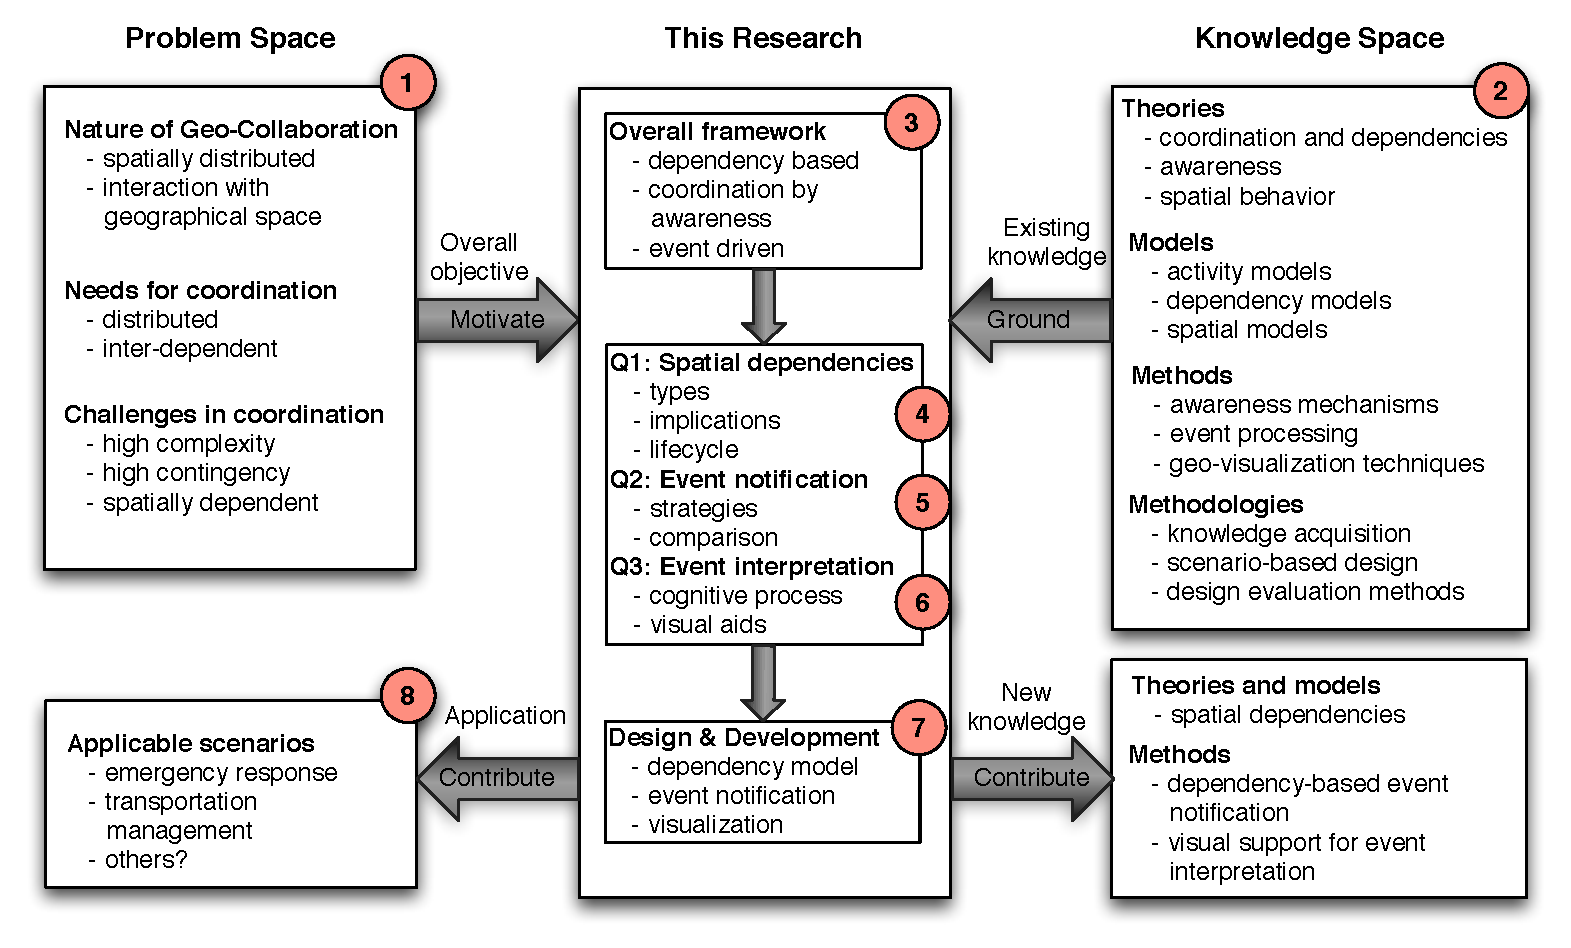
\includegraphics[width=5.8in]{research_overview.pdf} 
   \caption{Overview of the research approach}
   \label{fig:research_overview}
\end{figure}

% section research_objectives (end)

\section{Thesis Structure} % (fold)
\label{sec:thesis_structure}
The rest of this document is structured corresponding to how each chapter fits into the overall research framework. Chapter 2 presents the grounding work of this study, including the various studies on awareness phenomena. Chapter 3 provides the overall design framework and used it to review existing studies. Chapter 4-7 provide the details of our approach to awareness promotion. Chapter 8 demonstrates the use of the approach in several cast studies. Chapter 9 concludes the study.
% section thesis_structure (end)
